En primer lugar se tuvo que diseñar y construir un prototipo que respondiese a una serie de exigencias impuestas por el experimento. Por un lado  debía de ser capaz de albergar de manera segura  un haz de 35 fibras centelleadoras, el cual se encontraría totalmente sumergido en una solución de agua tritiada estanca. Este prototipo debía de ser capaz de comunicar los extremos del haz con fotosensores, los cuales deben estar aislados del agua tritiada, sin que existiese ningún tipo de fisura para asegurar que no existe peligro de fuga y, por tanto, de contaminación, ni siquiera por evaporación del agua. Por otro lado debía de sostener de forma segura el fotosensor utilizado, en nuestro caso PMTs, para leer la señal recibida por estas fibras centelleadoras.

Con todas estas exigencias, el material elegido para la construcción del prototipo fueron diversos elementos de fontanería de PVC. El motivo de este es su seguridad, ya que están especialmente diseñados para transportar  agua, su facilidad de manipulación ya que podemos realizar cortes con mucha rapidez, sencillez y eficacia además de existir muchas formas para diversos fines disponibles en el mercado y, finalmente, su precio, ya que se trata de un material bastante económico. 

En concreto, se adquirió un tubo de PVC de $2~\meter$ de longitud y un diámetro interior de $15~\milli\meter$, en el cual se practicaron una serie de cortes, dando lugar a un conjunto de secciones que conformarían los 2 prototipos. Para unir cada una de estas secciones y dar forma al prototipo, se utilizaron codos, típicamente utilizados en fontanería de PVC, cuyas uniones serían finalmente selladas mediante soldadura química. Finalmente el prototipo quedaría sujeto de forma segura sobre una estructura de metacrilato y acero. El aspecto final del prototipo puede verse reflejado en la figura 20.

\begin{figure}[hbtp]
\centering
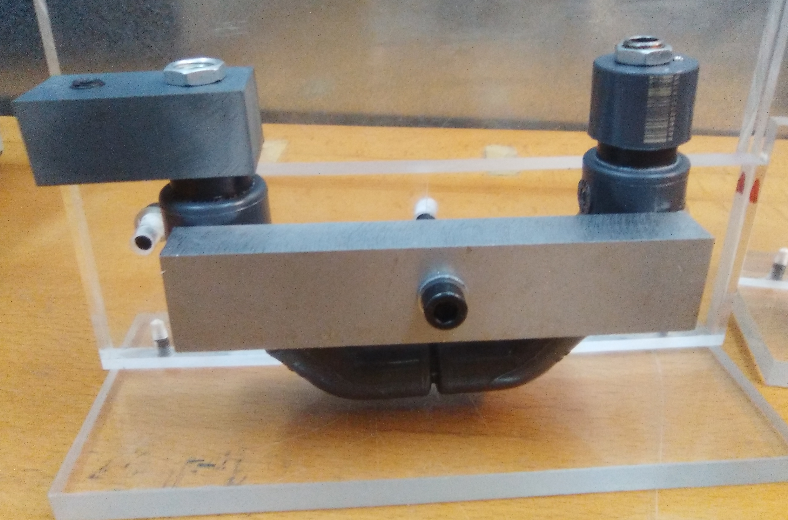
\includegraphics[scale=0.3]{Prototipo.png}
\caption{ Prototipo\label{prototipo}}
\end{figure}

Este prototipo tiene un volumen interior que permite rellenarlo con   $39~\cm^3$ de solución radiactiva, el cual se calculó y verificó con varios ensayos de llenado con agua destilada. También se verificó la estanqueidad del prototipo mediante ensayos de 2 días. 

Se decidió realizar un prototipo con forma de U. Dado que el prototipo no se trasladará en ningún caso y, teniendo en cuenta que se verificó su estanqueidad, personalmente opino que esta es la forma más segura y que mejor se adapta a las exigencias del prototipo. Las dos oberturas superiores se cerraron  y selladaron con tapones, unos utilizados en fontanería de PVC y otros fabricados para este prototipo en los talleres mecánicos del IFIC. Se eligieron tapones diferentes para cada extremo. Un primer tapón circular,  correspondiente al tubo de PVC y un segundo tapón cuadrado, diseñado para facilitar el proceso de llenado. Este segundo tapón dispone de  un orificio de 8 mm por el que se realizó el proceso de llenado  mediante una pipeta. Al otro tapón  se le ha practicado  un orificio de $1~\milli\meter$ para purgar el aire durante el  proceso de llenado. Finalmente estos orificios se cerraron con  tornillos de rosca envueltos en teflón, finalmente se sellaron con silicona. Estos tapones se muestran en la figura~\ref{tapones}.

Además ambos extremos disponen también de un agujero de $9.8~\milli\meter$ de diámetro, tamaño justo para que por cada uno de estos pasara un extremo del haz de fibras centelleadoras. En estos extremos se dispusieron dos arandelas, roscadas al aro que conformaba el extremo del haz, según la figura~\ref{prototipo} (una arandela a cada extremo del tapón, parte interior y exterior). De esta forma conseguíamos fijar perfectamente cada uno de los extremos del haz al prototipo y comunicar el extremo de las fibras al exterior del prototipo para su correspondiente lectura con los fotosensores, PMTs en nuestro caso. 



También podemos observar que se ha decidido realizar el giro de $180\degree$, correspondiente a la U, con ayuda de cuatro codos de $45\degree$ y no con dos codos de $90\degree$. Esto es debido a que, con giros progresivos, el haz de fibras centelleadoras están sometidos a una tensión inferior y, por extensión, ofrecerán una mejor propagación de la señal.

Finalmente se utilizaron dos piezas, usualmente utilizadas en fontanería de PVC para comunicar tuberías de igual o diferente diámetro para sostener los PMTs en el prototipo. Debido al hecho de haber utilizado dos tapones distintos ahora necesitaremos dos piezas diferentes. Estas pueden verse en la figura 21.

\begin{figure}[hbtp]
\centering
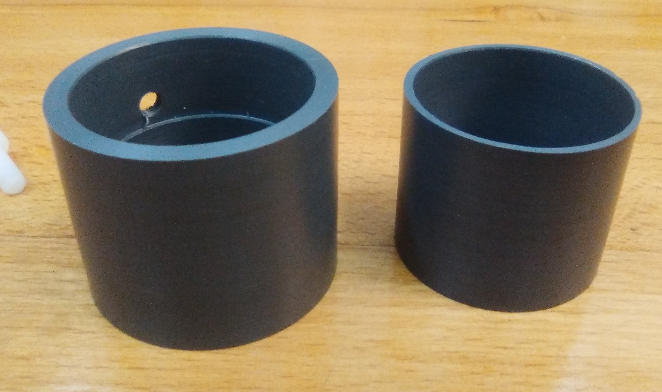
\includegraphics[scale=0.4]{Tapones.png}\\
\caption{ Piezas de sujeción de los PMTs\label{tapones}
}
\end{figure}

La primera pieza (correspondiente a la pieza derecha de esta figura), más pequeña, simplemente encajaba al tapón circular por un extremo y, por el otro, con un diámetro interior más grande para que cupiese y fijase, se disponía del PMT.

Para la segunda pieza encontramos un problema y es que no hay tuberías cuadradas, por lo que no encontramos ningún tipo de pieza  que ajustase a este tapón (tapón cuadrado del prototipo). En su lugar simplemente utilizamos una pieza para que encajase a la arandela que sobresalía del prototipo (utilizada para fijar el haz de fibras) y por el otro extremo que encajase al PMT. Para mejorar la sujeción se utilizó en esta pieza un tornillo que unía ésta al soporte de metacrilato. La disposición de los PMT en el prototipo y el tornillo que ayuda a la sujeción pueden verse  en  la figura~\ref{prototipotapones}.

\begin{figure}[htb]
\centering
{
%\subfloat[Espectro de emisión]
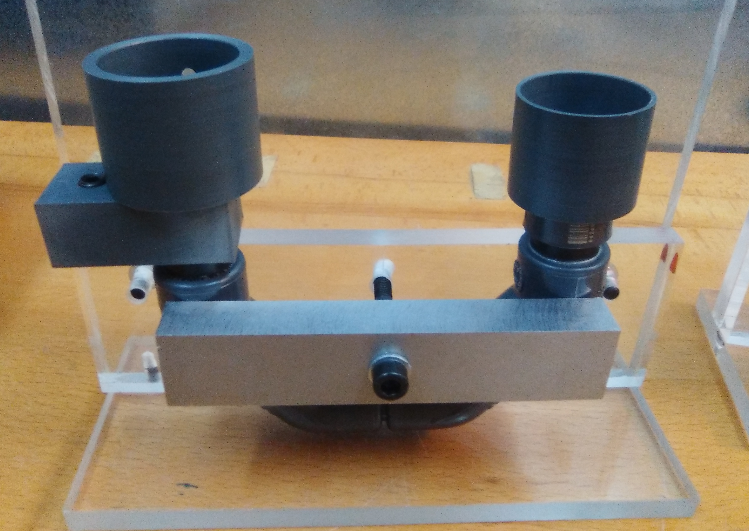
\includegraphics[scale=0.25]{Prototipodelantetapon.png} 
}
{
%\subfloat[Espectro de emisión]
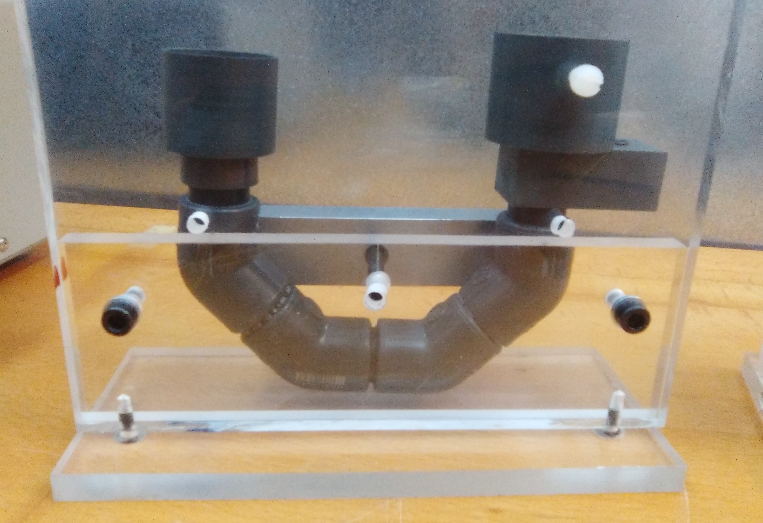
\includegraphics[scale=0.25]{PrototipoDetrastapon.png} 
}
\caption{Prototipo con piezas de sujeción \label{prototipotapones}}
\end{figure} 

Hay que tener en cuenta que el proceso de medida se desarrollará en el interior de una cámara oscura, cuya única labor es la de proteger de la posible entrada de luz del exterior. En esta no habrá un control exhaustivo de la temperatura como ocurría con el sistema utilizado para la calibración de los SiPM. En su lugar únicamente activaremos el aire acondicionado en la sala para mantener una temperatura constante de aproximadamente $25~\celsius$ en todo momento.

Los PMTs empleados, R8520-ZB2771 y R8520-ZB2773 se alimentaron ambos a $-830~\volt$ . A esta temperatura disponen de una ganancias de $G_1=1456178$ y $G_2=1921595$ y sus eficiencia de fotodetección a $\lambda=430~\nano\meter$ son del $29.76\%$ y $28.66\%$, respectivamente. 
